\section{Discussion on Incremental Confidence and Independence Assumptions}

Historically, \cref{ax:funcform} has not proved as anodyne as it looks.
Some might object that it's not possible to write such a function that is appropriate in all circumstances.
For example, Shafer argues for Dempster's rule of combination as a way of incorporating information, but is very careful to emphasize that it ought to be used only on \emph{independent} information, for reasons illustrated below.



\begin{example}
    % \label{ex:dupl}
	You have initial belief state $\theta_0$.
	Now, someone comes up to you and tells you that $\phi$ is true, a statement
		that you trust to some intermediate degree of confidence $c \notin\{ \bot, \top\}$.
	So, in accordance with \Cref{ax:funcform}, you use $F$ to transform your beliefs, partially incorporating the information to arrive at some belief state $\theta_1 := F^c_\phi(\theta_0)$.
	Immediately afterwards, your friend repeats what they just said: $\phi$ is true.
	Your confidence in the statement remains the same, and so according to
	\Cref{ax:funcform}, you again update your beliefs, arriving at $\theta_2 := F^c_\phi(\theta_1)$.
	Except in very special circumstances (e.g., you already know that $\phi$ is true, or $c \in \{\bot,\top\}$), typically $\theta_2$.
	And yet, it seems your your attitude towards $\phi$ ought to be the same whether you've heard it twice or only once.
\end{example}


Now, it's important to mention that we're not quite in the same position as Shafer.
Shafer was prescribing a concrete representation of $\Theta$ (a belief function) and a concrete update rule $F$ (Dempster's rule of combination), and so he needed to defend these choices.
% To take an analogous prescriptive stance,
We only need to defend something much more modest: we only need to defend the assumption that, if $\Theta$ and $\Phi$ properly model the relevant aspects of the scenario at hand, then there exists \emph{some} function $F$ which performs updates appropriately.
Descriptively speaking, we're also in good shape: for synthetic agents, it suffices to point out that learning algorithms represent functions, which given a state, an input, and a number of iterations (confidence), produce an output.
And, supposing that $\Theta$, $\Phi$, and $\confdom$ all capture the relevant respective aspects of a human's belief state, input information, and attitude towards it, how could it be that a human does otherwise?
%
% After all, if you recieve the same input twice, and your confidence in it has not changed, it would be best to only update once.
% There are essentially three ways to proceed.
In any case, keeping \cref{ex:dupl} in mind, here are three ways to proceed.

\begin{enumerate}[label={\textbf{I\arabic*.}},ref={I\arabic*}]
	\item \textbf{Accept Severe Limiations.} \label{approach:assume}
	Like Shafer, we could be careful
	% not to claim anything about how to update beliefs, except
	to claim nothing about the belief updating process except in the (unusual) case where
	information recieved is independent.
	% This severly handicaps the usefulness of .
	This would be a severe limiation to the theory, and much less necessary than it was for Shafer.
	Imagine that we are writing code that describes how a synthetic agent updates its beliefs. Shafer's approach is to package any such code with a warning against running it unless assured that observations will always be independent.
	But independece is notoriously difficult to establish; are we to simply accept that the code will not behave correctly in any realistic scenario?
	% Under what circumstances could we possibly be sure that all inputs we will be independent?

	In practice, many theoretical properties of standard statistical learning algorithms are heavily dependent on indepencence assumptions (most commonly, that one recieves independent, identically distributed samples).
	% Despite this, such algorithms .
	This warning label not seem to keep them from being applied in settings where practitioners readily admit samples are not really independent at all---nor indeed performing well emperically in those settings \parencite{???}.

	% If we need to make a decision that depends on information that is not given, then
	% Shafer found himself in a position where he needed to qualify usage of the update rule


	\item \textbf{Appropriately Enrich Domains.}\label{approach:enrich}
	% For instace, the agent has been totally
	% We told a story wanting to avoid incorporating information twice.
	In \cref{ex:dupl}, it seems obvious that we ought to ignore the second copy of the information, because it has already been accounted for.
	However, this intuition is highly contingent on the implicit supposition that we \emph{know} the second input to be a replica of the first.
	Were we ignorant to the nature of the second piece of information, perhaps it would not be so unreasonable to incroproate it again, even without a proof of independence.
	% If we want our agent to do the same
	% In asking our agent to take such issues into account, it is only fair to give it access to the same
	% It seems unfair to criticize an agent for not behaving
	So, if we would like our agent to make the same decisions that we did, it seems only fair to give it access to the knowledge that we needed to get there.
	One way of doing this is to extend the belief state so that it also tracks what information has been incorporated.
	% For instance, suppose that every message

	For \cref{ex:dupl} to work, it is critical that we are able to discern that the two inputs were identical.
	As a result, it seems that the relevant description of the input information was not just $\phi$, but a pair $(\phi, \mathit{id})$ that also a description of its identity.
	It is also critical that we remember the identity of previously incorporated information, so we would also be better off with a belief space $\Theta$ reflects this.
	With these two modifications, any \cofunc\ can be straightforwardly modified to avoid the issue in \Cref{ex:dupl}.


	We submit that it is always possible to enrich the space of beliefs and observations in this way to track the relevant information, to resolve the issue.
	With a few more assumptions later on, we will be able to formalize the construction we just alluded to (\cref{ex:dupl-enriched}).

	\item \textbf{An Incremental Interpretation of Confidence.}
		\label{approach:interperet}
	Finally, we can get around the issue by interpreting a confidence $c \in \confdom$ not as an absolute measurement of confidence, but rather an incremental one.  This means viewing $c \in \confdom$ as the degree of \emph{additional} confidence we have in $\phi$, beyond whatever we have already incorporated into our beliefs.

	% This proposal immediately raises some important questions.
	This proposal might be concerning.
	% First, how
	One might worry that it's harder to make sense of ``incremental confidence'' than an absolute notion.
	How ought we to numerically describe the confidence of an update?
	Suddenly this becomes much more subjective, for to assign a number, not only must we describe how much trust we have in the new information, but we must also take history or current belief state into account.
	Furthermore, the words ``incremental'' and ``additional'' suggest that we will need a formal description of how to aggregate confidences---%
	the very concept of which we will need to defend.
	% Indeed, such a way of combining confidences will ultimately play a large role for us.
	% It will turn out that such a way of combining confidences
	% Fortunately, it will turn out that

	Even modulo these concerns, the incremental interpretation still leaves us in a strictly better place than we were before.
	%  with \cref{approach:assume}.
	To begin, in situations where inputs are independent (i.e., the only cases where we would have been allowed to apply the \cofunc\ according to \cref{approach:assume}), the two notions coincide.
	More explicitly: if the new information $\phi$ is indepenendent of everything we've previously seen, then an absolute measurement of our confidence in it is no different from a measrurement of how much we ought to increment it from having no confidence.
	Already, though, we can do more.
	In the situation described by \cref{ex:dupl}, for instance,
	the second utterance induce no \emph{additional} confidence ($\bot$), and so applying $F$ with no confidence clearly gives the desired result of ignoring the new information (per \cref{ax:zero}).
%
%
	And even in general, the prospect of having to numerically estimate a fuzzy quantity seems more promising than red tape requiring that $F$ only be used (in good conscience) on independent information.
	% In some ways, this approach it is not so different from directly requiring independence of inputs, there are several aspects of this framing, that in our view, make it more pallatable.
	% First,
	% In cases
	% This raises some questions. Even if we already had a

\end{enumerate}

We would like to point out that readers who find who find it reasonable to ignore inputs you have no confidence in (per \cref{ax:zero}) have implicitly either accepted either \cref{approach:assume} or \cref{approach:interperet}, as the next example shows. 


\begin{example}
	Suppose you first hear $\phi$ from a partially trusted source, and incroproate it into your beliefs appropriately.
	Then, the same source sends you a second message, which is obviously spam.
	In an absolute sense, you now have no confidence ($\bot$) in anything this source tells you, including (in retrospect) both messages.
	It seems appropriate to excise $\phi$ from your belief state in response, rather than leaving your belief state unchanged, as \cref{ax:zero} would prescribe.

	Note that in this scenario, while it seems that we ultimately have no confidence in $\phi$, it does not seem to be the case that we have no incremental confidence in $\phi$.
	Rather, the incremental confidence seems to be the inverse of the original confidence.
\end{example}

We state our results with the incremental interpretation of confidence, with the understanding that all of our results also admit a more conservative reading, in which confidence is measured absolutely, and also all applications of the function $F$ are independent. 

\section{Other Confidence Domains}

% \begin{phaseout}
To describe a degree of partial incorporation, we will need a domain of possible confidence values.
Mostly, we will stick to using real numbers, but it will clarify things to stay more general for now, so that we can see the properties we actually need.
% Formally, we represent the possible degrees of confidence by a group
Formally, a \emph{confidence domain} is a tuple $(\confdom, \oplus, \bot, \top)$,
where $(\confdom, \oplus, \bot)$ is a monoid with operation $\oplus$ and neutral element $\bot$, and $\top \in \confdom$ is an absorbing element---i.e., $\top \oplus c = \top$ for all $c \in \confdom$.
In terms of confidence, we interpret the components as follows:

\begin{itemize}%[]
	\item
	The elements of $\confdom$ are the possible degrees of confidence.

	\item
	The monoid operation $\oplus : \confdom \times \confdom \to \confdom$ describes how to combine two (independent) confidences in some statement, to obtain a new confidence in that statement.

	\item The neutral element $\bot \in \confdom$ indicates ``no confidence'' in an observation.
		%
		% The fact that we want to ignore information we have no confidence in
		% gives corresponds to the group identity laws: that
	The monoid identity laws, which assert that
		$\bot \oplus c = c = c \oplus \bot$ for all $c \in \confdom$,
	reflect the intuition that we should ignore untrusted information in combining confidences.
		% in which case we should ignore the information at hand,
	\item The absorbing element $\top$ indicates ``full confidence''.
	The absorbtion property corresponds to the intuition that, definitive information that $\phi$ is true, when combined with other (perhaps less reliable) information that $\phi$ is true, is still definitive.
\end{itemize}
% \end{phaseout}

In this more general setting, the analogue of additivity (\cref{ax:additivity}) becomes:
\begin{CFaxioms}
	\item For all $c_1, c_2 \in \confdom$,~
		% $F^{c_1}_\phi \circ F^{c_2}_\phi = F^{c_1 \oplus c_2}_\phi$
		$F^{c_1}_\phi \circ F^{c_2}_\phi = F^{c_1 \oplus c_2}_\phi$
		% \hfill \textbf{(additivity)} \label{ax:additivity}
		\hfill \textbf{(combination)} \label{ax:gen-combine}
\end{CFaxioms}
\Cref{ax:gen-combine}
 % looks like it could be problematic, but it
 simply states that \cofunc s respect the combination operation.
If we fix an assertion $\phi$, then an update with confidence $c_1$ followed by an update with confidence $c_2$ is equivalent to an update with confidence $c_1 \oplus c_2$, which is, by definition, the result of comining confidences $c_1$ and $c_2$.
On its own, so long as we have the freedom to choose $\confdom$, \Cref{ax:additivity} has no teeth.


\begin{prop} \label{prop:free-additivity}
	If $F: \confdom \to (\Phi \to (\Theta \to \Theta))$ satisfies \cref{ax:zero,ax:idemp}, then we can construct a new update
	% function for $\Theta$ on $\Phi$, that behaves in exactly the same way, but \emph{is} additive, but with the altered confidence domain
	function for $\Theta$ on $\Phi$, that behaves in exactly the same way, except that it is exteneded to a larger confidence domain, for which which it does satisfy \cref{ax:additivity}.
\end{prop}
\begin{lproof}
Consider the new confidence domain
$$
	\confdom' := \Big\{ \text{ finite lists } [c_1, \ldots c_n]
		\text{ with each } c_i \in \confdom,
		% \text{ such that } c_i \in \confdom \text{ for all } i = 1, \ldots, n
		\quad
		% \text{list concatenation}~::,
		::,
		\quad
		[\,],
		\quad
		[\top]
		\,
	\Big\},
$$
whose group operation ``$::$'' is list concatenation, except that it collapses instances of $\top$, i.e.,
\[
	[c_1, \ldots c_n] :: [d_1, \ldots, d_m]
	 := \begin{cases}
		 % [\top] & \text{ if } c_i = \top \text{ for some $i$ or $d_j=\top$ for some $j$}\\
		 [\top] & \text{ if } \top \in \{c_1, \ldots, c_n,d_1, \ldots,d_m \} \\
		 [c_1, \ldots, c_{n}, d_1, \ldots, d_m] & \text{otherwise.}
 \end{cases}
\]
Concatenating the empty list $[\,]$ on either side has no effect,
by construction, for all $L \in \confdom'$, we have $[\top] :: L = [\top] = L :: [\top]$,
and $::$ is clearly associative, so $\confdom'$ is also a confidence domain.

The new update rule for this confidence is given by:
	\[
		AF^{[c_1, \ldots, c_n]}_\phi (\theta)  :=
				(F^{c_n}_\phi \circ \cdots \circ F^{c_1}_\phi) (\theta).
	\]
$AF$ has the same behavior as $F$ on the elements that correspond to the original confidence domain, since
$
	AF^{[c]}_\phi(\theta) = F^c_\phi(\theta),
$
and it is additive by construction, since
\begin{align*}
AF^{[c_1, \ldots, c_n]}_\phi ( AF^{[d_1, \ldots, d_m]}_\phi (\theta) )
		&:=
			F^{d_m}_\phi \circ \cdots \circ F^{d_1}_\phi (
			F^{c_n}_\phi \circ \cdots \circ F^{c_1}_\phi (\theta))\\
		&= (F^{d_m}_\phi \circ \cdots \circ F^{d_1}_\phi \circ
		F^{c_n}_\phi \circ \cdots \circ F^{c_1}_\phi) (\theta) \\
		&= AF^{[c_1, \ldots, c_n, d_1, \ldots, d_m]}_\phi (\theta) \\
		&= AF^{[c_1, \ldots, c_n] :: [d_1, \ldots, d_m]}_\phi (\theta).
\end{align*}
\end{lproof}% We are primarily interested in the case where confidence can be measured as a real number,
For convenience of measurement, and so that we may better study confidence as a \emph{smooth} interpolation between ignoring and fully incorporation, we shall focus primarily on cases where confidence can be measured as a real number.
% We now define two confidence domains that are real numbers between 0 and 1.
We now consider two such confidence domains.

\begin{itemize}
	\item
	% Another confidence domain we could consider
	First, we consider the zero-one confidence domain
	\[
		\ZO := \Big(~ [0,1],
			% \quad a \star b := a b,
			\quad a \star b :=
					% 1- (1-a)(1-b) =
					a + b - ab,
			\quad 1,
			\quad 0 ~\Big),
	\]
	which uses the same numerical endpoints as probability;
	a value of zero represents no confidence, a value of one represents full confidence.
	For the purposes of updating, we may interpret a confidence of $a \in \ZO$ as the fration of the way between ignoring and fully incorporating information.
	This motivates the definition of the operator $\star$.
	If you go $90\%$ of the way to fully incorporaing some information $\phi$, and then $50\%$ of the remaining way, then in total you have gone $90\% + 50\%(100\%-90\%) = 0.9 + 0.5 - (0.9)(0.5)$ of the way to fully incorporating $\phi$.

	% In this domain
	% Clearly, 1 is neutral and 0 is absorbing element.\end{itemize}
	\item
	% First, we consider the monoid of positive extended real numbers under addition.
	We now introduce a second confidence domain based on the real numbers,
	which is mathematically cleaner, if
		% at first
		more difficult to interpret numerically in absolute terms.
	\[
		\Rplus :=
			\Big([0, \infty) \cup \{\infty\},
				\quad +,
				\quad 0,
				\quad \infty
				~\Big)
	\]

	% The use of addition as the combination operator means that independent measurements add, which in turn makes it
	The use of addition as the combination operator makes it particularly natural to speak of linear combinations of inputs.
	% Here are some examples.
	This point is best illustrated by example.

	\begin{itemize}
		\item \textbf{Voting.}
		Suppose the elements of $\Phi$ correspond to candidates in an election.
		In a sense, the number of votes a candidate recieves is a measure of how much confidence the electorate has in them---a candidate who recieves no votes is ignored, while a candidate who recieves all of the votes should be listened to exclusively.

		It's hard to say much  the raw number of votes a candidate recives in absolute terms, in part becasue it depends on the number of votes recieved by other candidates, and also how many votes you will recieve in the future.
		% Nevertheless, it is still m
		Nevertheless, if we are collecting votes, is especially natural to weight candidates by the total number of votes behind them.
		% Similarly, this way of counting fractional votes.
		This way of measuring confidence also applies without change to measure fractional votes.

		\item \textbf{Chemical Reactions.}
		Suppose that we have a mixture of nano-bots.
		Each nano-bot has some type $\phi \in \Phi$, and has the effect of turning matter into bots of type $\phi$.
		For every $\phi \in \Phi$, let $\beta_\phi$ be the concentration of bots of type $\phi$, say measured in number of bots per liter of solution.
		In some sense, $\beta_\phi$ measure of how much ``confidence'' the mixture has in $\phi$---if the concentration is zero, then that bot type may be ignored, and if all particles are of type $\phi$, then

		\TODO

		% Suppose that there is a chemical mixture of nano-bots. each of type $\phi_i$.

	\end{itemize}

	We will use greek letters $\alpha, \beta, \ldots$ to denote elements of $\Rplus$.

\end{itemize}


\begin{prop}
	$\ZO$ is isomorphic to $\Rplus$, but therere is no canonical choice of isomorphism.
\end{prop}
\begin{lproof}
	For every $k > 0$ can construct an isomorphism $\varphi_k: \ZO \to \Rplus$ explicitly by $\varphi(a) := - k \log a$.
	It is a homomorphism, since
	\[
		\varphi(a \star b) = - k \log (a b) = - k \log a - k \log b =
			\varphi(a) + \varphi(b),
	\]
	while $\varphi(1) = 0$ (so it preserves the identity) and $\varphi(0) = \infty$ (so it preserves the absorbing element).
	The inverse mapping can also be explicitly by $\varphi^{-1}(r) := \exp( - r / k)$, which is also a homorphism for the same reasons as above.
\end{lproof}


\section{Extra}

\subsection{Invertable Update Rules}

\begin{CFaxioms}
	\item For all $\phi\in\Phi$, and $\beta \in \mathbb R$, the update
	$F^{\beta}_{\phi}: \Theta \to \Theta$ is invertable.
	\hfill\textbf{(Invertability)} \label{ax:invert}
\end{CFaxioms}


This effectively partitions $\Theta$ into two


\begin{prop}
	If $F$ is a differentiable and invertable update rule (i.e., satisfies \cref{ax:zero,ax:additivity,ax:invert,ax:diffble}), then for all $\beta \in \mathbb R$, $\phi \in \Phi$, the function
	% $F^\beta_\phi : \Delta\X \to \Delta\X$
	$F^\beta_\phi : \Theta \to \Theta$
	is a diffeomorphism, and its inverse is given by $F^{-\beta}_\phi$, in the sense that
	\[
		F^{-\beta}_\phi( F^{\beta}_\phi (\mu) ) = \mu = F^{\beta}_\phi( F^{-\beta}_\phi (\mu) ).
	 \]
\end{prop}


% Together with strong additivity, we get
% \begin{prop% We are primarily interested in the case where confidence can be measured as a real number,
%     If $F$ is an update rule satisfying \cref{ax:additivity,ax:invert},
%     then any update prescribed by $F$ (or sequence thereof) takes positive distributions to positive distributions.
%     %
%     Concretely, for all $\beta$ and $\phi$,   $\mu \in \mathrm{Int}(\Delta\X)$ if and only if $F^{\beta}_\phi(\mu) \in \mathrm{Int}(\Delta\X)$.
%     If $F$ further satisfies \cref{ax:sufficiency, ax:diffble}, then
%     % \[
%         $F^\beta_\phi$ is a diffemorphism of $\mathrm{Int}(\Delta\X)$.
%     % \]
% \end{prop}


As a consequence,
\begin{coro}
	If for any $\beta < \infty$ there exist $\mu, \phi, A$ such that
	$\mu(A) > 0$  but $F^{\beta}_\phi(\mu)(A) = 0$, then $F$ is not invertable.
\end{coro}



\section{}
\begin{example}\label{ex:dupl-enriched}
Suppose $F$ is an additve update rule. Then, we can explicitly construct a resolution to the problem posed in \cref{ex:dupl} by defining enriched spaces
\begin{align*}
	\Phi' &:= \Phi \times \Big\{ \text{ identities }~ \mathit{id}~ \Big\}\\
	\Theta' &:= \Theta \times
		\Big\{ \text{histories } L = [(\phi_1, \mathit{id}_1, c_1), \ldots (\phi_n, \mathit{id}_n, c_n)] \Big\} \\
\end{align*}
and new \cofunc\ $G$ by
\begin{align*}
	 G^{\beta}_{(\phi,\mathit{id})}(\theta, L) & :=
		\begin{cases}
		\Big( F^{\beta- \sum_{i}\beta_i \mathbbm1[(\phi_i,\mathrm{id}_i) = (\phi, \mathrm{id})]}_{\phi}(\theta),~
			 L :: (\phi,\mathit{id}, \beta)
		 \Big)
			 &\text{ if } \beta \ne \bot \\
		(\theta, L) &
			   \text{ if } \beta = \bot
	\end{cases}
\end{align*}
\end{example}


\section{More on Path Update Rules}
Since each $\phi$ corresponds to a path

\begin{defn}[Homotopic update rules]
	$\phi \sim_F \psi$  iff 
	they behave the same way for full confidence (that is, 
	$F^1_{\phi}(\theta) = F^1_{\psi}(\theta)$ for all $\theta \in \Theta$)
	and  there exists a continuous function
	$H : \Theta \times [0,1] \times [0,1]$ such that,
	for all $\theta \in \Theta$ and $\chi \in [0,1]$,
	\begin{enumerate}[nosep]
		\item $H(\theta, \chi, 0)= F(\theta, \chi, \phi)$,
		\item $H(\theta, \chi, 1)= F(\theta, \chi, \psi)$
	\end{enumerate}
	and for all $s \in [0,1]$,
	\begin{enumerate}[nosep,resume]
		\item $H(\theta, 0, s) = \theta$;
		\item $H(\theta, 1, s) = F^1_{\phi}(\theta) = F^1_{\psi}(\theta)$,
		the last two of	which are the same by assumption. \qedhere
	\end{enumerate}
\end{defn}

As usual, homotopy is an equivalence relation.

For example, the Dempster-Shafer update rule \eqref{eq:ds-prob} is homotopic 
to the linear update rule from \cref{ex:prob-simple}. 


\section{Proofs}

\recall{theorem:add-reparam}
\begin{lproof}\label{proof:add-reparam}
    
\end{lproof}

\section{More Examples}


Next, and example in which we have an additive flow update rule,
that is not an optimizing update rule, and hence has no loss representation.

\begin{example}[Weighted Average]
    Suppose we recieve vectors $\phi \in \mathbb R^n$, 
    say estimates of a quantity from different sources.
    Suppose further that our belief state
    $(\mat x,w) \in \Theta$ consists a current estimate
    $\mat x$ of the quantity of interest, and a weight $w$ of the total internal confidence in the estimate.
    In other words:    
	\begin{align*}
		\Theta = \mathbb R^n \times [0,\infty];
		\qquad
        \text{and}
        \qquad
		\Phi = \mathbb R^n %; \qquad
        .
	\end{align*}

	Updating proceeds by taking a weighted average of the previous estimate and the new input, weighted by their respective confidences, which is captured by:
	\begin{align*}
		F^\beta_{\mat y}(\mat x, w) &=  \left( \frac{ w \mat x + \beta \mat y}{w + \beta} , w + \beta \right)
		\qquad\text{and}\qquad
		F^{\beta}_{\mat y}(\mat x, \infty) = (\mat x, \infty)
	\end{align*}
	It is additive, since
	\begin{align*}
		&F^{\beta_2}_{\mat y} \circ F^{\beta_1}_{\mat y}(\mat x, w) \\
		&= \left( \frac{ (w + \beta_1) \frac{ w \mat x + \beta_1 \mat y}{w + \beta_1} + \beta_2 \mat y}{(w + \beta_1) + \beta_2}, (w  + \beta_1) + \beta_2 \right) \\
		&= \left( \frac{  w \mat x + (\beta_1 + \beta_2) \mat y}{w + (\beta_1 + \beta_2)}, w  + (\beta_1 + \beta_2)\right)
		= F^{\beta_1 + \beta_2}_{\mat y}(\mat x, w).
	\end{align*}
	And it is clearly differentiable, with a simple calculation revealing that
	$ F'_{\mat y}(\mat x, w) = \left( \frac{\mat y - \mat x}{w}, 1\right) $.

	Observations:
	\begin{itemize}
		\item The update rule cannot be extended differentiably to states $\theta = (\mat x, w)$ with $w = 0$.
			Intuitively, we need to have some estimate with positive confidence to update beliefs in a differentiable way.
        This is related to the fact that plain emperical risk minimization (ERM) is unstable, but stable with even a small amount of regularization.
			% It is also similar to the fact that one needs a prior in order to do
			% In this case, the prior may be arbitrarily weak.
		\item The certainties are given by
		\[
			\lim_{\beta \to \infty} F^{\beta}_{\mat y}(\mat x, w) = (\mat y, \infty)
		\]
		% \item In this case,
		\item $F$ is commutative, invertible, and symmetric with respect to permutation of the dimensions, but it is not conservative: if we had $U(\mat x, w, \mat y)$ twice differentiable such that $\nabla_{\mat x, w} U = F'$, then we would have
        \begin{align*}
        \frac{\partial^2}{\partial w \partial x_i} U &=
			\frac\partial{\partial w} \frac{y_i - x_i}{w} = \frac{x_i - y_i}{w^2},\quad\text{but}
            \\
		\frac{\partial^2}{\partial x_1 \partial w} U
			&= \frac\partial{\partial x_i} 1 = 0    
        \end{align*}
		violating Clairaut's theorem (which asserts equality of mixed partials).
		Therefore, $F'$ cannot be written as the gradient of a function,
        and so $F$ is not an optimizing update rule. \qedhere
	\end{itemize}
\end{example}

Next, a toy example that showcases an assortment of other features and themes that can be captured with our definition of confidence.

\begin{example}\label{ex:jugo}
% \def\Gpressed(#1,#2){\mathsf{G}_{#1}\text{-}\mathit{pressed}(\mathsf{G},#1,#2)}
% \def\Gpressed(#1,#2){\mathit{pressed}(#1,\mathsf{G},#2)}
\def\pressed(#1,#2,#3){\mathit{pressed}(#1,\mathsf{#2},#3)}
Jugo is an impartial juror.
Like the other jurors, she has two buttons in front of her,
labeled $\sf G$ and $\sf N$.
% The button labeled $\mathsf G$ increases the probability 
% of a guilty verdict, while the button labeled $\mathsf N$ increases
% the probability of a not-guilty verdict. 
Her instructions are to listen to evidence, and press $\sf G$ to 
increase the probability of a guilty verdict, and $\sf N$ 
to increase the probability of a not-guilty verdict.

More concretely, the system works as follows.
There are $J$ jurors, labeled $\{1, \ldots, J\}$;
let 
% $G_j(t)$ be
$\pressed(j,B,t)$ be
a variable that is equal to one if juror $j \in $
is pressing button  $\mathsf B$ button at time $t$, and zero otherwise.
% ; symmetrically, let $N_j(t)$ indicate whether $j$ is pressing the $\mathsf N$ at time $t$.
The ``belief state'' of this automated system is
a single number $g \in [0,1]$, representing the probability of a guilty verdict.
When a single juror presses $\mathsf G$, $g$ approaches 1
exponentially, and if they instead press $\sf N$, $g$ decays to zero.
In the first case ($\sf G$ is pressed) the system evoves according to 
$\frac{\mathrm dg}{\mathrm dt} = (1-g)$
while in the second, 
$\frac{\mathrm dg}{\mathrm dt} = -g$.
The first is the vector field associated with the $\mathsf G$ button,
and the second is the vector field associated with $\sf N$. 
The total effect of all buttons is then the sum of that of all buttons across all vector fields, when they are active:
% in which case $g(t) = 1 + (g(0) - 1)e^{-t} $.
% Concretely, their dynamics are governed by:
\[
	\frac{\mathrm dg}{\mathrm dt} = 
	\sum_{j = 1}^J 
		% G_j(t)
		\pressed(j,G,t)
		(1-g) 
		-
		% N_j(t)
		\pressed(j,N,t)
		(g)
		~,
	% \begin{cases}
	% 	(1 - p)	& \text{button $\uparrow$ pressed} \\
	% 	-p & \text{button $\downarrow$ pressed}
	% \end{cases}	
\]
so that $g$ exponentially approahces $1$ when more $\mathsf G$ buttons are pressed than $\mathsf N$ buttons,
and symmetricaly, exponentially approaches $0$ when more $\mathsf N$ buttons than $\mathsf G$ buttons are pressed.
At the end of the trial, the defendant is convicted with probability
equal to the final value of $g$. 

Let $\phi$ represent a piece of evidence suggesting guilt, presented by the
prosecution from time $t_1$ to time $t_2$,
and suppose for now that only buttons labeled $\mathsf G$ are pressed
in this interval.
% Many aspects of this scenario can be understood in terms of confidence.
%
	% The amount of time that 
	% What is the confidence of the system in that evidence, as it understands it from the Jurors?
% First, suppose that only $\mathsf G$ buttons are pressed
	 % between $t_1$ and $t_2$. 
% in between times $t_1$ and $t_2$.
The system measures $j$'s confidence in $\phi$ by
\[
	w_j := \!\int_{t_1}^{t_2}\!\! G_j(t) \mathrm d t 
	= \text{ total time $j$ presses $\mathsf G$ during $\phi$,}
\]
Note that $w_j = 0$ if and only if $j$ does not press any buttons,
which (a) indicates that $j$ does not trust the evidence $\phi$, 
and (b) communicates this fact to the system, by telling it to ignore 
the evidence. 
Note that this is an additive representation of confidence, since
pressing the button for four seconds, and then three more later, is
by definition the same as pressing it for seven. 
While the maximum possible confidence of $w_j$ is $(t_2 - t_1)$,
this system does not allow a juror to express \emph{full} confidence in $\phi$
because no finite amount of $\mathsf G$-pressing will result in a 
guilty verdict with probability one; it is always possible to increase
the value of $g$ through additional evidence. 

% Now, recall that ,
Altogether, the system's confidence in $\phi$ can be measured by
as the unique value $W$ for which
\begin{align*}
	% \int_{t_1}^{t_2} W (1-g(t)) \mathrm d t = \int_{t_1}^{t_2} \sum_{j=1}^J G_j(t) (1-g(t)) \mathrm d t,
	\int_{t_1}^{t_2} W (1-g(t)) \mathrm d t =
	 g(t_2) - g(t_1),
	% \\
	% W = \frac{1}{t_2-t_1 - \int_{t_1}^{t_2}g(t) \mathrm dt} \int_{t_1}^{t_2} \sum_{j=1}^J G_j(t) (1-g(t)) \mathrm d t
\end{align*}
which, so long as only $\mathsf G$ buttons are pressed, equals
$W := \sum_{j} w_j$, so this measure of confidence is additive 
across jurors as well as across time. 
This is appropriate, since the jurors are independent and 
not communicating with each other.
% This is a weighted sum of $w_i's$
As before, $W = 0$ if and only if no juror presses any buttons between times $t_1$ and $t_2$,
indicating zero trust leant to $\phi$. In such a case, the system ignores $\phi$ in updating its beliefs.
And just as no individual juror can send a full-confidence update to the system,
	the system cannot recieve a full-confidence from the jurors as a whole.
	
The picture gets significantly more complicated if we consider the possibility
that jurors might press the $\mathsf N$ button. For example, if $\phi$, which was intended
as evidence of guilt, has the effect of getting jurors to press $\mathsf N$, there is a sense
in which they have \emph{negative} confidence in $\phi$, since the belief update happened in the opposite direction of what $\phi$ represents; rather than \emph{no} trust, this is represents \emph{distrust}. 
Small negative updates are always possible except at the boundary of belief space, but in this paper, we focus almost entirely on positive confidence updates.

The introduction of the second button also uncovers a significant source of complexity:
unlike \cref{ex:prob-simple,ex:classifier,ex:shafer}, 
the order that evidence is presented matters, when there is more than one possible response to it.
Evidence presented later has a larger effect,
meaning that this system exhibits a recency bias.
% (This lack of commutativity corresponds to possibility that,
%	as a Lie algebra, the bracket may not be identically zero.)

Now consider a variant of this system that does
not trust all jurors equally; rather, it trusts each juror $j$
to a degree $\beta_j \in [0, \infty]$, and now $g$ evolves
according to
\[
	\frac{\mathrm dg}{\mathrm dt} = 
	\sum_{j = 1}^J \beta_j \Big( G_j(t) (1-g) 
		- g N_j(t) \Big).
	% \begin{cases}
	% 	(1 - p)	& \text{button $\uparrow$ pressed} \\
	% 	-p & \text{button $\downarrow$ pressed}
	% \end{cases}	
\]
In this case, the system can be said to have trust $\beta_j$ in juror
$j$, since $j$'s buttons are ignored when $\beta_j = 0$. 
When $\beta_j = \infty$ (an expression of full confidence in $j$),
$g$ immediately jumps to 0 when $j$ presses 
$\mathsf N$, or to 1 if $j$ presses $\mathsf G$ (unless canceled by
another full-confidence juror pressing the opposite button).
If all jurors have full confidence, then the verdict of this system is
a majority vote at the last moment a button was pressed. 
Thus, the weights attached to weighted combinations are (additive) expressions 
of confidence as well. 
\end{example}

\section{Counter-Examples}

\subsection{Nonmonotonic Updates (Dropping \ref{ax:seq-for-more})}
    % strangely, doesn't work with \cref, or \ref* or \cref*.
Without \cref{ax:seq-for-more}, we could have a situation like the below,
in which resuming an update could take you to a completely different position
if you were interrupted in the middle of the path. 

\begin{center}
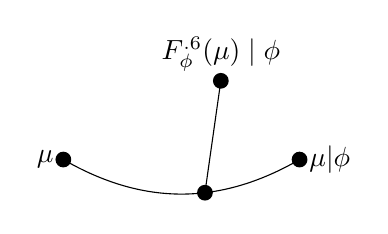
\begin{tikzpicture}
    \coordinate[label=left:$\mu$] (A) at (0,0);
    \coordinate[label=right:$\mu|\phi$] (C) at (3,0);
    \coordinate[label=above:$F_\phi^{.6}(\mu)\mid\phi$] (C') at (2,1);
    \draw (A) to[bend right] node[outer sep=0,pos=0.6](B){} (C);
    \fill 
        (A) circle (0.1)
        (B) circle (0.1)
        (C) circle (0.1)
        (C') circle (0.1);
    \draw (B.center) to (C');
\end{tikzpicture}
\end{center}


\subsection{Halting Updates (Dropping \ref{ax:nopause})}
The next two examples further explore the motivation behind \cref{ax:nopause}

\begin{example}
Suppose $\Theta = \mathbb R \cup \{-\infty, \infty\}$, $\Phi = \{\star\}$ is a singleton, and
and 
\[
    F^t_{\!\star}(\theta) = \theta + t + \sin(t).
\]

This is interesting because it ``pauses'' 
Clearly $F$ satisfies \cref{ax:zero,ax:idemp,ax:cont,ax:diffble}.
It also satisfies \cref{ax:seq-for-more}, since it is increasing in $t$
(but it is not additive \cref{ax:additivity}).
%
Its vector field is given by 
\[
    \frac{\partial}{\partial t} F^t_{\!\star}(\theta) = 1 + \cos(t) \Big|_{t=0}
     = 2,
\]
so its unique additive representation is
$
    {^+}F^t_{\!\star}(\theta) = \theta + 2 t.
$
\end{example}

\begin{example}
Now suppose $\Theta$ and $\Phi$ are as before,
but now
\[
    F^t_{\!\star}(\theta) = \theta + t - \sin(t).
\]
As before, it satisfies \cref{ax:zero,ax:idemp,ax:cont,ax:diffble,ax:seq-for-more},
but now its vector field is
\[
    \frac{\partial}{\partial t} F^t_{\!\star}(\theta) = 1 - \cos(t) \Big|_{t=0}
     = 0,
\]
so its unique additive representation does nothing:
$
    {^+}F^t_{\!\star}(\theta) = \theta. 
$
\end{example}

\subsection{}
